% LTeX: language=it

\chapter{Architettura del compilatore}
\label{chap:architettura-del-compilatore}

Nel seguente capitolo si descrive l'architettura del compilatore BugginOut, affrontando i moduli che lo compongono e le fasi del compilatore che realizzano.

\begin{figure}[H]
	\centering
	\scalebox{0.75}{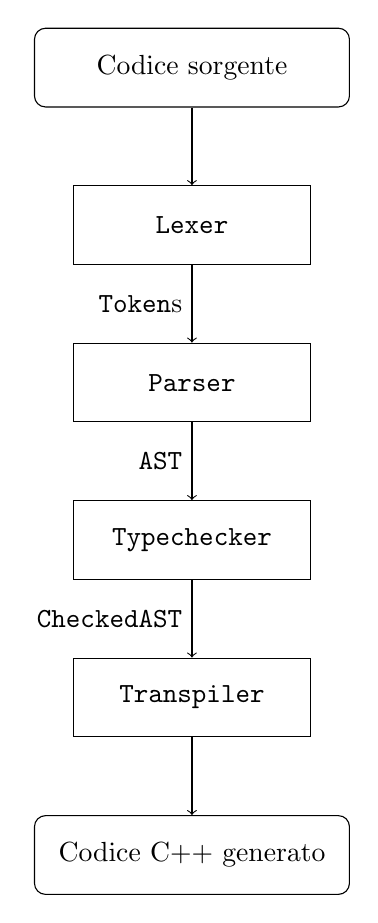
\begin{tikzpicture}[node distance=2cm]
		\node (source) [draw, rectangle, text centered, minimum width=4cm, minimum height=1cm, rounded corners] {Codice sorgente};
		\node (lexer) [below of=source, draw, rectangle, text centered, minimum width=3cm, minimum height=1cm] {\texttt{Lexer}};
		\node (parser) [below of=lexer, draw, rectangle, text centered, minimum width=3cm, minimum height=1cm] {\texttt{Parser}};
		\node (typechecker) [below of=parser, draw, rectangle, text centered, minimum width=3cm, minimum height=1cm] {\texttt{Typechecker}};
		\node (transpiler) [below of=typechecker, draw, rectangle, text centered, minimum width=3cm, minimum height=1cm] {\texttt{Transpiler}};
		\node (output) [below of=transpiler, draw, rectangle, text centered, minimum width=4cm, minimum height=1cm, rounded corners] {Codice C++ generato};

		\draw [->] (source) -- (lexer);
		\draw [->] (lexer) to node[left] {\texttt{Token}s} (parser);
		\draw [->] (parser) to node[left] {\texttt{AST}} (typechecker);
		\draw [->] (typechecker) to node[left] {\texttt{CheckedAST}} (transpiler);
		\draw [->] (transpiler) -- (output);
	\end{tikzpicture}}
	\caption{Moduli del processo di compilazione}
	\label{fig:moduli-compilatore}
\end{figure}

Nella figura sopra si pu\`o osservare l'architettura ad alto livello del compilatore che \`e costituito da quattro moduli principali:
\begin{itemize}
	\item \texttt{Lexer}: realizza l'analisi lessicale;
	\item \texttt{Parser}: realizza l'analisi sintattica;
	\item \texttt{Typechecker}: realizza l'analisi semantica;
	\item \texttt{Transpiler}: realizza la generazione del codice C++.
\end{itemize}
Questi interagiscono secondo un modello a \textit{pipeline}, in cui l'output di un modulo \`e l'input del successivo. Nel seguito si descriver\`a ciascuno di questi moduli e ci\`o che producono.

\section{\texttt{Lexer}}
\label{sec:lexer}

\begin{figure}[H]
	\centering
	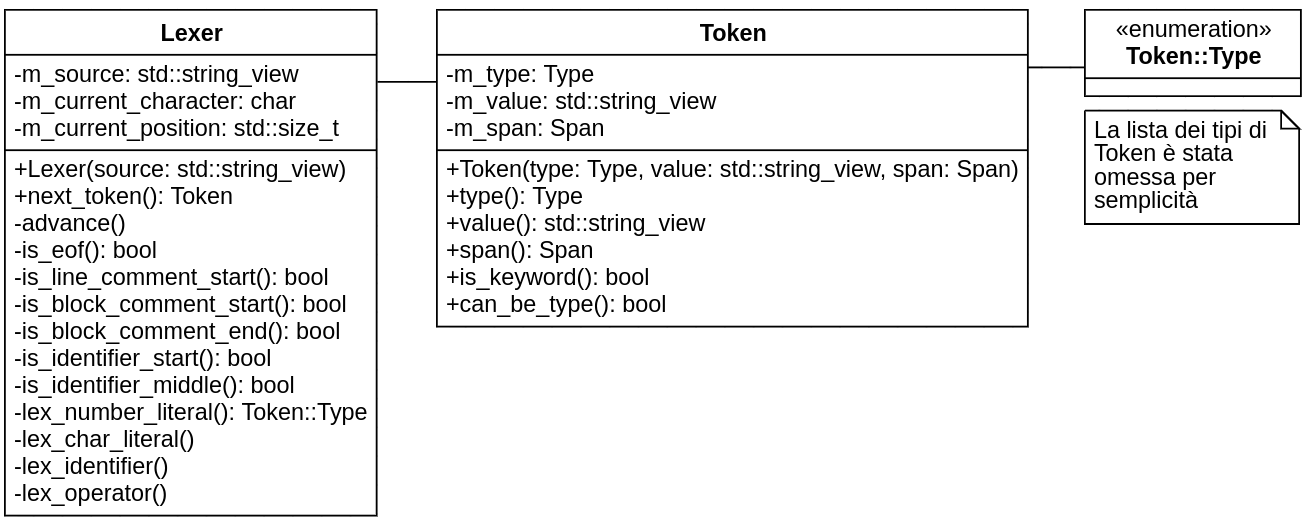
\includegraphics[width=0.8\textwidth]{figures/lexer.png}
	\caption{Diagramma UML del \texttt{Lexer}}
	\label{fig:lexer-uml}
\end{figure}

L'analisi lesicale \`e realizzata attraverso la classe \texttt{Lexer}. Questo \`e una classe che viene costruita
